% ECO387C Macro I, Fall 2026 - mock midterm Question 1, written up in the
% same form as the PSet 6 solutions (pset-06-solutions.tex). Author: Philip
% Livdan. Stochastic endowment economy, identical agents, riskless bond,
% two-state Markov endowment with state-specific stay probabilities p_h, p_l.
% Numbers are checked in mock-midterm-checks.py (mock-midterm-checks.txt).
% Notation follows the mock: a_{t+1} bond bought at t, gross rate R_t,
% y in {y_h, y_l}, stay probabilities p_h and p_l, CRRA gamma.
% Introduced by me: b := R_{t-1} a_t, R(y), pi(y'|y).
\documentclass[12pt]{article}
\usepackage{amsmath,amssymb}
\usepackage[margin=1.1in]{geometry}
\usepackage{tikz}
% float (vendored in ~/tools/tectonic/texmf) for [H].
\usepackage{float}
% Local tectonic cache lacks the 5pt and 6pt math fonts (cmmi6.pfb, cmsy5.pfb);
% keep script/scriptscript math at 8pt/7pt at every text size that uses math.
\DeclareMathSizes{12}{12}{8}{7}
\DeclareMathSizes{11}{11}{8}{7}
\DeclareMathSizes{10}{10}{8}{7}
% The cache has no monospace fonts at all: render code in roman.
\renewcommand{\ttdefault}{lmr}
\setlength{\parindent}{0pt}
\setlength{\parskip}{0.5\baselineskip}
\allowdisplaybreaks
\newcommand{\E}{\mathbb{E}}

\title{Mock Midterm, Question 1 Solutions\\[1mm] \large ECO387C Macro I, Fall 2026}
\author{Philip Livdan}
\date{October 6, 2026}

\begin{document}
\maketitle

\textbf{Acknowledgment.} I solved every problem by hand on paper. The
handwritten pages were then scanned and typeset with ChatGPT so that the
LaTeX is readable, and I checked the typeset version against my notes.
The numbers are checked in \texttt{mock-midterm-checks.py}, with output in
\texttt{mock-midterm-checks.txt}.

$u(c)=\frac{c^{1-\gamma}}{1-\gamma}$, $u'(c)=c^{-\gamma}$, and the transition probabilities are
\[
  \pi(y_h\mid y_h)=p_h,\quad \pi(y_l\mid y_h)=1-p_h,\qquad
  \pi(y_l\mid y_l)=p_l,\quad \pi(y_h\mid y_l)=1-p_l
\]
(Azzimonti et al., Section 7.1.2, p.\ 193).

\section*{Part (a): flow budget constraint}

\[
  c_t+a_{t+1}=R_{t-1}a_t+y_t ,
\]
plus a no-Ponzi condition, which does not bind in Part (e).

\section*{Part (b): state variables}

$(b_t,y_t)$ with $b_t:=R_{t-1}a_t$. $y_t$ is income, forecasts $y_{t+1}$
(Markov, $p_h\neq1-p_l$), and prices the bond, $R_t=R(y_t)$. Identical
agents make the bond distribution degenerate, so no other aggregate state
is needed.

\section*{Part (c): Bellman equation}

With $c=b+y-a'$ and $b'=R(y)a'$,
\[
  V(b,y)=\max_{a'}\Big\{\frac{(b+y-a')^{1-\gamma}}{1-\gamma}
  +\beta\sum_{y'\in\{y_h,y_l\}}\pi(y'\mid y)\,V\big(R(y)a',\,y'\big)\Big\},
\]
that is,
\begin{align*}
  V(b,y_h)&=\max_{a'}\Big\{u(b+y_h-a')+\beta\Big[p_h\,V\big(R(y_h)a',y_h\big)+(1-p_h)\,V\big(R(y_h)a',y_l\big)\Big]\Big\},\\
  V(b,y_l)&=\max_{a'}\Big\{u(b+y_l-a')+\beta\Big[(1-p_l)\,V\big(R(y_l)a',y_h\big)+p_l\,V\big(R(y_l)a',y_l\big)\Big]\Big\},
\end{align*}
as in Section 7.6, p.\ 219, with $q=1/R(y)$.

\section*{Part (d): Euler equation}

FOC in $a'$ (interior), using $\partial b'/\partial a'=R(y)$,
\[
  -u'(b+y-a')+\beta R(y)\,\E\big[V_b(R(y)a',y')\mid y\big]=0 .
\]
Envelope, with policy $a'=g(b,y)$,
\begin{align*}
  V_b(b,y)&=u'(c)\Big(1-\frac{\partial g}{\partial b}\Big)
  +\beta R(y)\,\E\big[V_b(b',y')\mid y\big]\frac{\partial g}{\partial b}\\
  &=u'(c)+\frac{\partial g}{\partial b}\Big[-u'(c)+\beta R(y)\,\E\big[V_b(b',y')\mid y\big]\Big]
  =u'(c),
\end{align*}
the bracket being zero by the FOC. Update one period and substitute,
\[
  u'(c)=\beta R(y)\,\E\big[u'(c')\mid y\big],
  \qquad\text{i.e.}\qquad
  c_t^{-\gamma}=\beta R_t\,\E_t\big[c_{t+1}^{-\gamma}\big].
\]

\section*{Part (e): market clearing and the equilibrium rate}

Goods and bonds clear,
\[
  \int c_t=y_t,\qquad \int a_{t+1}=0 .
\]
Identical agents facing the same $R_t$ choose the same $a_{t+1}$, so bond
clearing gives $a_{t+1}=0$, and the budget gives $c_t=y_t$ (Section 7.5,
p.\ 217). $R$ solves the Euler equation at $c=y$,
\[
  R(y)=\frac{u'(y)}{\beta\,\E[u'(y')\mid y]}
  =\frac{y^{-\gamma}}{\beta\sum_{y'}\pi(y'\mid y)\,(y')^{-\gamma}} .
\]

\section*{Part (f): rates with gamma = 2}

$u'(2)=\frac14$, $u'(1)=1$.
\begin{align*}
  \E\big[u'(y')\mid y_h\big]&=p_h\cdot\frac14+(1-p_h)\cdot1=\frac{p_h+4-4p_h}{4}=\frac{4-3p_h}4,\\
  R_h&=\frac{1/4}{\beta(4-3p_h)/4}=\frac1{\beta(4-3p_h)} .\\[2mm]
  \E\big[u'(y')\mid y_l\big]&=p_l\cdot1+(1-p_l)\cdot\frac14=\frac{4p_l+1-p_l}{4}=\frac{1+3p_l}4,\\
  R_l&=\frac{1}{\beta(1+3p_l)/4}=\frac4{\beta(1+3p_l)} .
\end{align*}
\[
  \boxed{\ R_t=\begin{cases}\dfrac1{\beta(4-3p_h)}, & y_t=y_h,\\[3mm]
  \dfrac4{\beta(1+3p_l)}, & y_t=y_l.\end{cases}\ }
\]
\textbf{Example,} $\beta=0.95$, $p_h=0.8$, $p_l=0.6$,
\[
  R_h=\frac1{0.95\cdot1.6}=\frac1{1.52}=0.658,
  \qquad
  R_l=\frac4{0.95\cdot2.8}=\frac4{2.66}=1.504,
\]
against $1/\beta=1.053$. For $p_h<1$, $4-3p_h>1$, and for $p_l<1$,
$1+3p_l<4$, so
\[
  R_h<\frac1\beta<R_l .
\]
Expected consumption growth is negative in a boom, so the rate that stops
saving is low, and positive in a recession, so the rate is high
(Figure~\ref{fig:R}).

\begin{figure}[H]
\centering
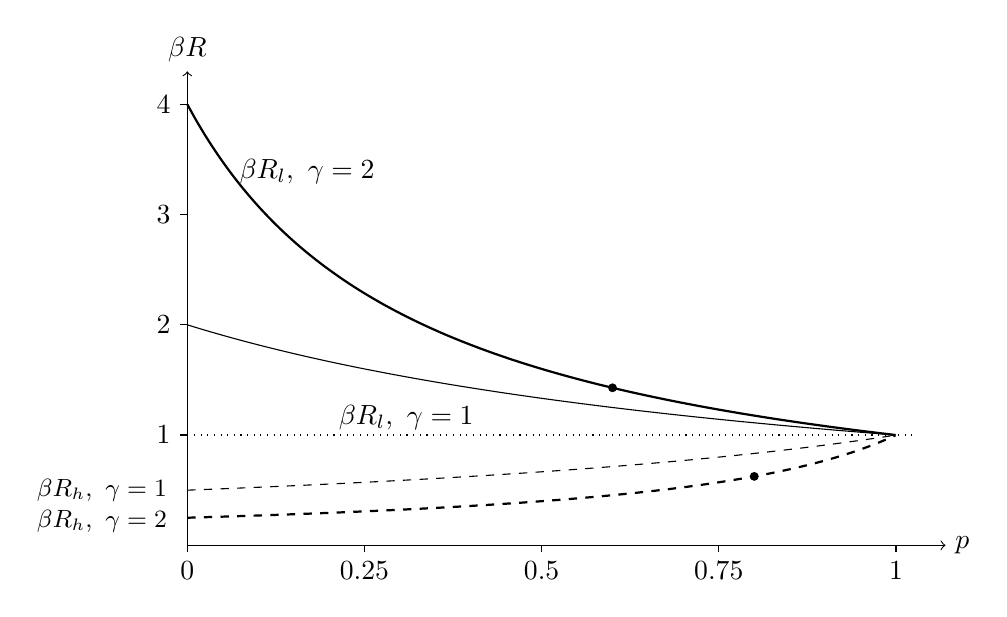
\begin{tikzpicture}[x=9cm,y=1.4cm]
  \draw[->] (0,0) -- (1.07,0) node[right]{$p$};
  \draw[->] (0,0) -- (0,4.3) node[above]{$\beta R$};
  \foreach \t in {0,0.25,0.5,0.75,1} \draw (\t,0) -- (\t,-0.06) node[below]{$\t$};
  \foreach \t in {1,2,3,4} \draw (0,\t) -- (-0.01,\t) node[left]{$\t$};
  \draw[dotted] (0,1) -- (1.03,1);
  \draw[thick] plot[domain=0:1,smooth,samples=80] (\x,{4/(1+3*\x)});
  \draw[thick,dashed] plot[domain=0:1,smooth,samples=80] (\x,{1/(4-3*\x)});
  \draw plot[domain=0:1,smooth,samples=80] (\x,{2/(1+\x)});
  \draw[dashed] plot[domain=0:1,smooth,samples=80] (\x,{1/(2-\x)});
  \node[right] at (0.06,{4/(1.18)}) {$\beta R_l,\ \gamma=2$};
  \node[anchor=north west] at (0.2,1.36) {$\beta R_l,\ \gamma=1$};
  \node[left] at (-0.015,0.5) {\small$\beta R_h,\ \gamma=1$};
  \node[left] at (-0.015,0.22) {\small$\beta R_h,\ \gamma=2$};
  \fill (0.6,{4/2.8}) circle (1.6pt);
  \fill (0.8,{1/1.6}) circle (1.6pt);
\end{tikzpicture}
\caption{Equilibrium gross rate times $\beta$ against the stay probability
of the current state, $y_h=2$, $y_l=1$. Solid, recession (horizontal axis
$p_l$). Dashed, boom (horizontal axis $p_h$). Thick, $\gamma=2$. Thin,
$\gamma=1$. The dotted level is $\beta R=1$. Dots mark the example,
$p_l=0.6$ and $p_h=0.8$ with $\gamma=2$.}
\label{fig:R}
\end{figure}

\section*{Part (g): curvature and the iid case}

The ratio of marginal utilities across states is
\[
  \frac{u'(1)}{u'(2)}=2^{\gamma}=2\ (\gamma=1),\qquad 4\ (\gamma=2).
\]
Higher $\gamma$ (lower IES $1/\gamma$) makes the same endowment change a
larger change in marginal utility, so the rate that supports $c=y$ moves
further from $1/\beta$. Same numbers with log utility,
\[
  R_h=\frac1{0.95\cdot(2-0.8)}=0.877,\qquad R_l=\frac1{0.95\big(0.6+0.4\cdot\frac12\big)}=1.316 .
\]
\textbf{iid,} $p_h=1-p_l$. Then $\pi(y_h\mid y_h)=\pi(y_h\mid y_l)=p_h$, so
\[
  \E\big[u'(y')\mid y_h\big]=\E\big[u'(y')\mid y_l\big]=p_h\,u'(2)+(1-p_h)\,u'(1)=:m,
\]
\[
  \frac{R_l}{R_h}=\frac{u'(1)/(\beta m)}{u'(2)/(\beta m)}=\frac{u'(1)}{u'(2)}=\frac{1}{1/4},
  \qquad
  \boxed{\ \frac{R_l}{R_h}=4\ }
\]
for any $p_h$, $p_l$, $\beta$. Example $p_h=0.4$, $p_l=0.6$: $R_h=0.376$, $R_l=1.504$.

\textbf{No trade is optimal.} $c_t=y_t$, $a_{t+1}=0$ satisfies the budget
and the Euler equation, consumption is bounded so transversality holds, and
$u$ is concave.

\section*{Sources}

\begin{itemize}\itemsep2pt
\item Azzimonti, M., P.\ Krusell, A.\ McKay, and T.\ Mukoyama (2024),
  \emph{Macroeconomics}, draft. Section 7.1.2 (Markov chains, p.\ 193),
  Section 7.5 (zero asset position of a representative household, p.\ 217),
  Section 7.6 (recursive consumption-savings problem, first-order and
  envelope conditions, Euler equation, pp.\ 218--219).
\end{itemize}

\end{document}
